\documentclass[border=8pt]{standalone}
\usepackage[utf8]{inputenc}
\usepackage{tikz}
\usetikzlibrary{shapes.geometric, positioning}

\tikzset{
  entita/.style     = {rectangle, draw, thick, fill=blue!8, minimum width=28mm, minimum height=9mm, font=\small},
  debole/.style     = {entita, double, double distance=1.5pt},
  relazione/.style  = {diamond, draw, thick, fill=orange!15, aspect=2.2, inner sep=1pt, font=\scriptsize},
  card/.style       = {font=\scriptsize, midway, fill=white, inner sep=1.5pt},
  link/.style       = {thick}
}

\begin{document}
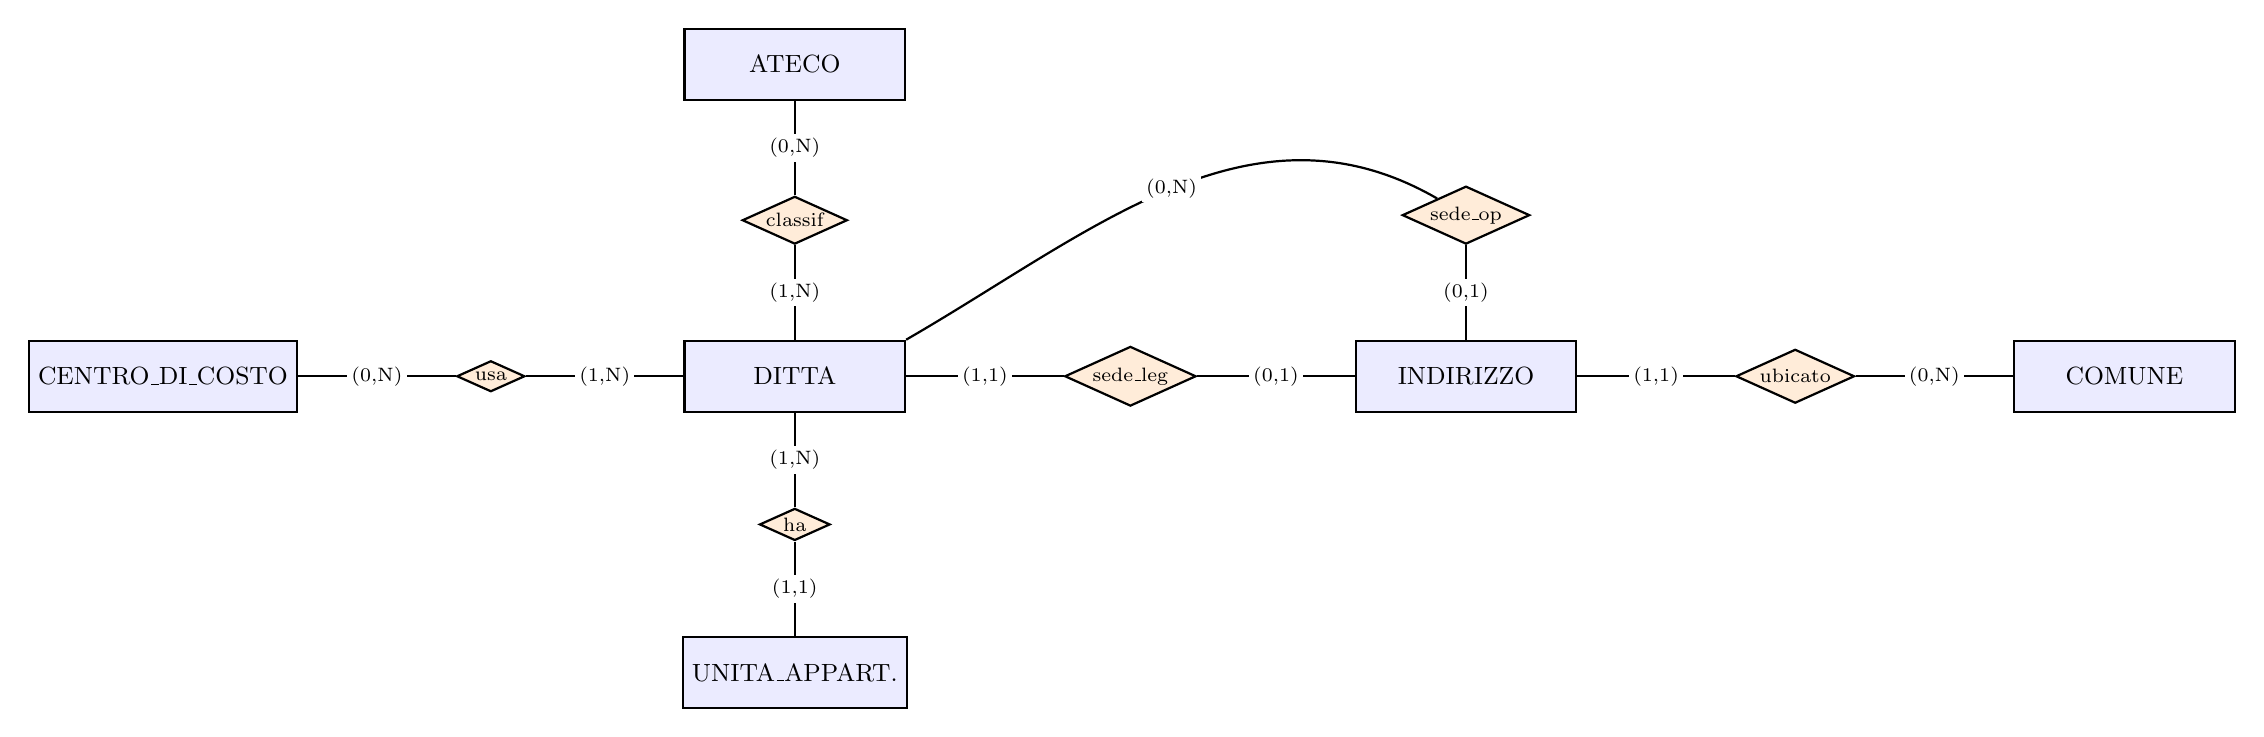
\begin{tikzpicture}[node distance=12mm and 20mm]

  \node[entita] (ditta) {DITTA};

  % ATECO (sopra, N:N)
  \node[relazione, above=of ditta] (classif) {classif};
  \node[entita, above=of classif]  (ateco)   {ATECO};

  % CENTRO_DI_COSTO (sinistra alto, N:N)
  \node[relazione, left=of ditta]  (usa)      {usa};
  \node[entita, left=of usa]       (cdc)      {CENTRO\_DI\_COSTO};

  % UNITA (basso sinistra, 1:N)
  \node[relazione, below=of ditta] (hau)      {ha};
  \node[entita, below=of hau]      (unita)    {UNITA\_APPART.};

  % INDIRIZZO + COMUNE (destra)
  \node[relazione, right=of ditta] (sedeleg)  {sede\_leg};
  \node[entita, right=of sedeleg]  (indir)    {INDIRIZZO};
  \node[relazione, above=of indir] (sedeop)   {sede\_op};
  \node[relazione, right=of indir] (ubic)     {ubicato};
  \node[entita, right=of ubic]     (comune)   {COMUNE};

  \draw[link] (ditta) -- (classif) node[card]{(1,N)};
  \draw[link] (classif) -- (ateco)  node[card]{(0,N)};

  \draw[link] (ditta) -- (usa)     node[card]{(1,N)};
  \draw[link] (usa) -- (cdc)       node[card]{(0,N)};

  \draw[link] (ditta) -- (hau)     node[card]{(1,N)};
  \draw[link] (hau) -- (unita)     node[card]{(1,1)};

  \draw[link] (ditta) -- (sedeleg) node[card]{(1,1)};
  \draw[link] (sedeleg) -- (indir) node[card]{(0,1)};
  \draw[link] (ditta.north east) to[out=30,in=150] node[card]{(0,N)} (sedeop);
  \draw[link] (sedeop) -- (indir)  node[card]{(0,1)};
  \draw[link] (indir) -- (ubic)    node[card]{(1,1)};
  \draw[link] (ubic) -- (comune)   node[card]{(0,N)};

\end{tikzpicture}
\end{document}
